\chapter{Simulation of a Plenoptic 2.0 System}
\markboth{\MakeUppercase{Simulations of a Plenoptic 2.0 System}}{}
\label{chap:chapter5}
This chapter describes the simulations done to characterize the optical performances of a focused plenoptic imaging system. The scope of this work is to investigate the behaviour of a plenoptic 2.0 imaging system at its diffraction limit under a wave optics approach.  All simulations described in this chapter have been run using the Fresnel Simulation Toolbox  described in chapter \ref{chap:fresnel}. In a plenoptic 1.0 imaging system the resolution is limited by the dimensions of the lenslets \cite{georgiev2009resolution} and the final rendered image has a much lower resolution then a conventional image. In a focused plenoptic system, as explained in section \ref{sec:phase2.0}, the resolution of the final rendered image is not linked any more to the number of lenslet in the micro array and it is possible to recover the full sensor resolution pushing it even to sub-pixel resolution \cite{lumsdaine2008full,lumsdaine2009focused,georgiev2009superresolution}. This characteristic makes plenoptic systems suitable to a wider range of applications where high spatial resolution is required \cite{wetzstein2011computational}. In the past years further effort has been made to push plenoptic 2.0 system to achieve super-resolution performances \cite{georgiev2012super,georgiev2009superresolution,bishop2009light}. Here the term super-resolution is not referred to the achievement of a resolution beyond diffraction limit\cite{georgiev2015plenoptic} but to a digital sub pixel resolution only. When applied to microscopy diffraction still represents a big limitation for plenoptic imaging systems. This chapter will discuss how diffraction affects the optical resolution of an imaging system and how it is linked to the spatio-angular trade off \cite{georgiev2006spatio}. Numerical simulations will be implemented using by the platform described in chapter \ref{chap:fresnel}. 
\label{sec:intro4}
\section{Rendering in Plenoptic 2.0}
\label{sec:rendering}
As introduced in chapter \ref{chap:chapter1}, rendering an image form plenoptic 2.0  raw data is based on integrating for each position all the correspondent directional coordinates. While in plenoptic 1.0 each position is sampled by a single lenslet, which causes the loss of resolution in the final image, in plenoptic 2.0 each position is sampled by several lenslets. Therefore with reference to figure \ref{fig:render202}, the spatial coordinate (x,y) of point $A$ will be sampled by the lenslets 1, 2 and 3, therefore $A$ is represented by 3 sub images. Each sub image is a different point of view of A and directional coordinates are sampled by these three points of view simultaneously. The number of sub images into which the point \textit{A} is imaged depends on the magnification \textit{m=b/a} of the lenslet array and is given by:
\begin{equation}
\label{eq:point_of_view}
N_{sub} = \dfrac{1}{m}=\dfrac{a}{b}
\end{equation}
 \textit{a} is the distance of the micro array from the main lens image and \textit{b} is the distance of the from the sensor plane. 
\begin{figure}[H]
	\centering
	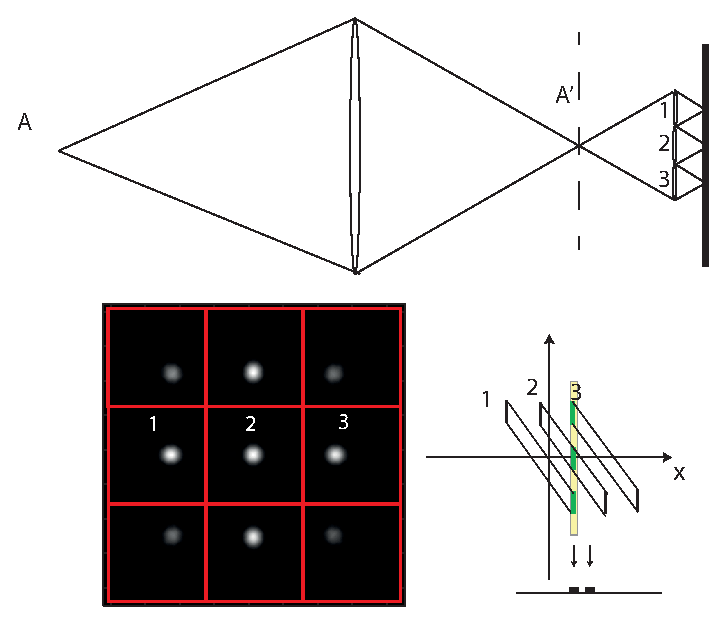
\includegraphics[width=.8\textwidth]{C:/Users/Massimo/Documents/Thesis/rendering201a.eps}
	\caption{\label{fig:render202} Top: the point $A$ is imaged by the main lens into the point $A'$. It is imaged by the lenslet array into a number of sub images depending by the magnification of the micro array stage, in this case \textit{m=0.333}. Bottom: particular of the raw image of the point source $A$ and phase space diagram. The three sub images \textit{1, 2} and \textit{3} are three different points of view of the object.  }
\end{figure}
From a computational point of view the basic rendering is performed directly on the raw sensor image and has the following steps:
\begin{itemize}
	\item the single sub images are isolated from each other 
	\item depending on the magnification \textit{m} the number of angular samples to be extracted from each sub image is calculated.
	\item the angular samples are extracted from the sub image and tiled all together forming the rendered image.
\end{itemize}
\subsection{Extracting Sub Images}
\label{sec:isolating}
The effects of distortion must be taken into account when extracting the sub images from the raw data.
The radial distortion is due to the fact that the sub images are shifted of a certain amount because the lenslets are imaging off axis. The shift is proportional to the distance from the centre of the micro array \cite{pedrotti1993introduction} hence the effects of this distortion are larger on the sub images at the edges of the raw data sub images array. These sub images are therefore misaligned with respect to the regular square grid of the micro lens array. 
With reference to figure \ref{fig:grid}:
\begin{equation}
 \label{eq:pincushio1}
\dfrac{x}{z+a}=\dfrac{x'}{b}
\end{equation}
Therefore each sub image under the lenslet is shifted of a quantity:
 \begin{equation}
 \label{eq:pincushion2}
 x' = \dfrac{xb}{z+a}
 \end{equation}
 Since $z \approx z+a$ each sub image is shifted by a quantity equal to:
\begin{equation}
\label{eq:pincushion}
x' = x\dfrac{b}{z}
\end{equation}
\begin{figure}[H]
	\centering
	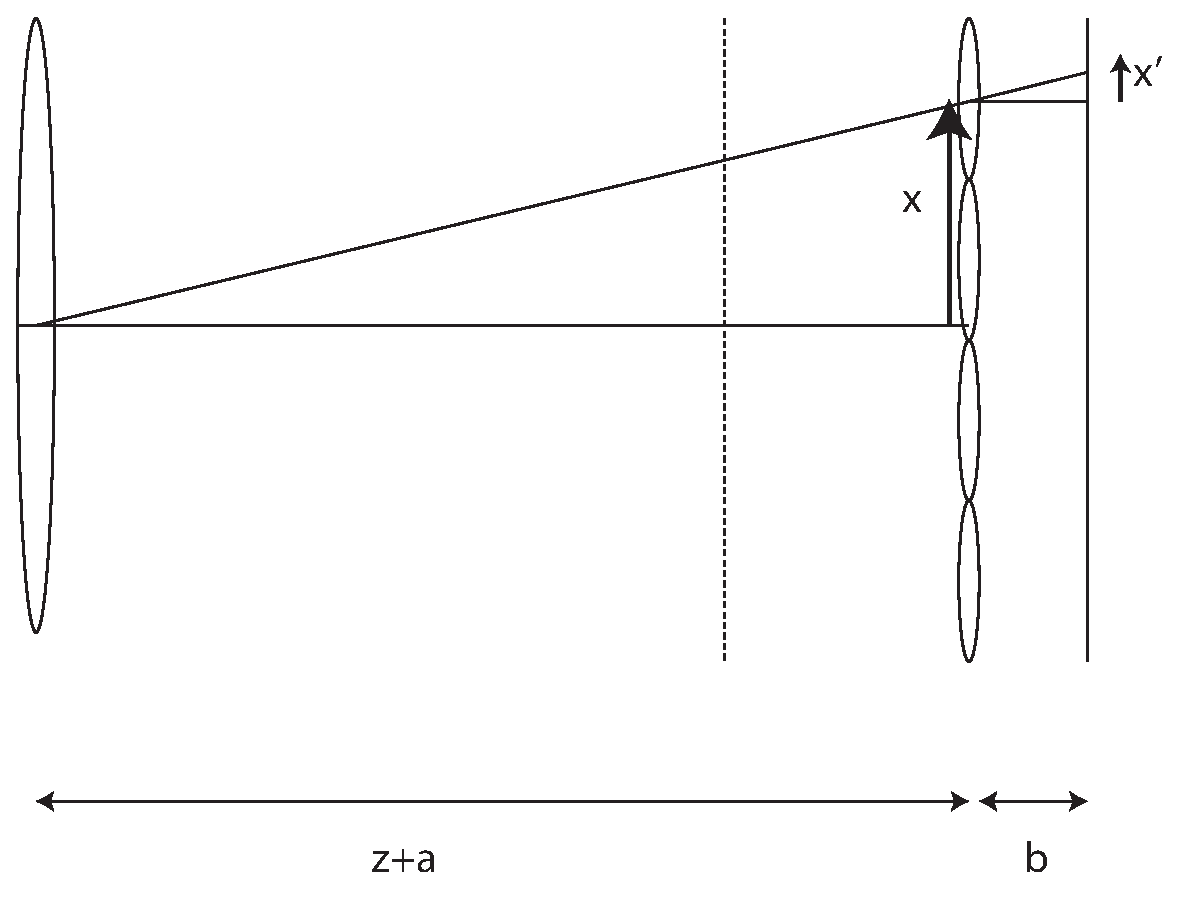
\includegraphics[width=.6\textwidth]{C:/Users/Massimo/Documents/Thesis/grid.eps}
	\caption{\label{fig:grid} Relation between the position of the centre of a lenslet \textit{x} and the position of the centre of the correspondent sub image $x + x'$.  }
\end{figure}
In figure \ref{fig:grid} \textit{x} is the position of the centre of a micro lens and its corresponding sub image will be shifted of a quantity $x'$ which depends on the distance of the image plane from the main lens \textit{z} and the distance of the sensor from the micro lens \textit{b}. Once the centres of the sub images have been localized it is possible to extract each sub image from the raw data and perform the rendering.
\subsection{Basic Rendering}
\label{sec:basicrendering}
This section will describe how the basic rendering algorithm works as seen in section \ref{sec:rendering201} and as described by Georgiev and Lumsdaine  \cite{georgiev2010focused,lumsdaine2009focused}.
The raw image on the sensor plane is an image of the main lens image plane \cite{georgiev2010focused}. Each sub image represents a single point of view of an area of the main lens image plane. Referring to figure \ref{fig:render20b}, if the micro array is composed of N $\times$ N lenslets, the raw sensor image will be composed of an N $\times$ N array of sub-images. Each sub-image has a dimension of P $\times$ P where P is the micro lens pitch. 
\begin{figure}[H]
	\centering
	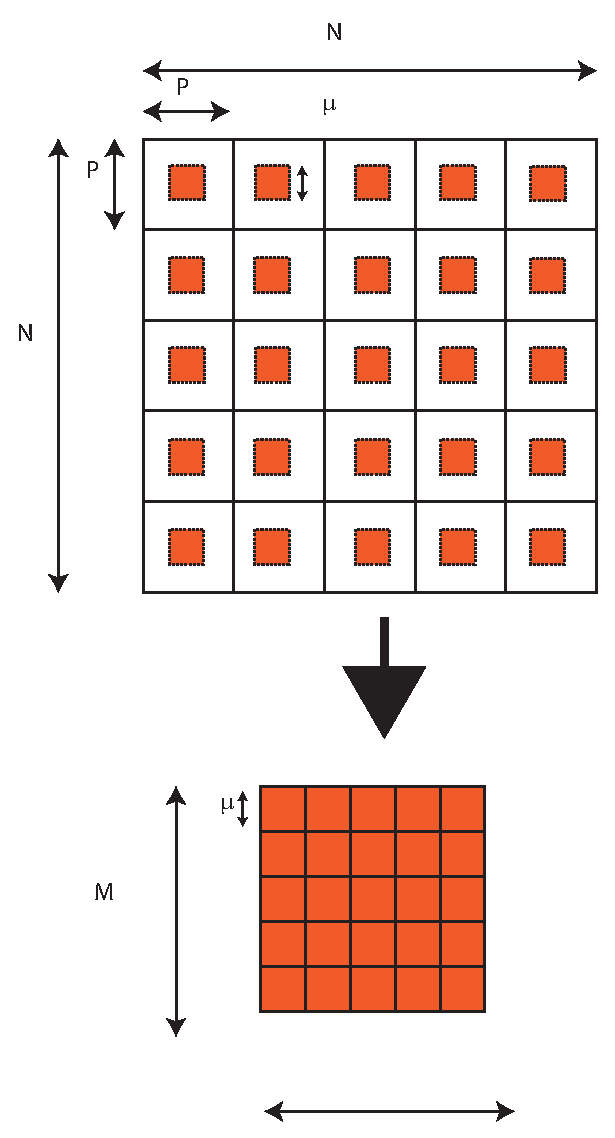
\includegraphics[width=.6\textwidth]{C:/Users/Massimo/Documents/Thesis/basicrendering.eps}
	\caption{\label{fig:render20b} Basic rendering algorithm. The Rendered image is made by tiling together patches extracted by each sub image. The patch size is dependent on the magnification of the micro array stage.  }
\end{figure}
The magnification of the micro array is \textit{m=b/a} and each micro lens maps the main lens image on the sensor plane on a sub image magnified by a quantity \textit{m}. Therefore from each sub image a patch is selected with a dimension equal to:
\begin{equation}
	\label{eq:patch}
	\mu = P \dfrac{b}{a} = P m
\end{equation}
The patch size depends on the magnification of the lenslets array. The next section will demonstrate how this fact can be used to recover depth information from the raw sensor images. 
\subsection{Depth Based Rendering}
\label{sec:depthbased}
The patch size $\mu$ as seen in equation \ref{eq:patch} depends on the magnification of the micro array stage. If the point imaged is out of focus, its image will be formed on a different plane that is not the main lens image plane. Hence the main lens image will be blurred and so will be the sub images on the sensor. If during the rendering process the fact that a point at a different depth with respect to the main lens focal plane will be imaged at a different distance from the micro lens array is taken into account. Therefore it is possible to define a new value of magnification $m'$ to which will correspond a new patch size $\mu'$.
Rendering with the new patch size allows refocusing at a different plane.\\
 With reference to figure \ref{fig:def20}, the points that belong to the plane shown represented by the dashed red line placed at a distance \textit{d} from the object plane, will be imaged on a plane in between the main lens and the main lens image plane. It is possible to define a virtual micro array stage with respect to this plane for which its points will be imaged in focus on a virtual sensor plane. The parameters characterizing the virtual micro array stage are the distances $a' $ and $b' $ and a magnification $m' = b'/a'$.
\begin{figure}[H]
	\centering
	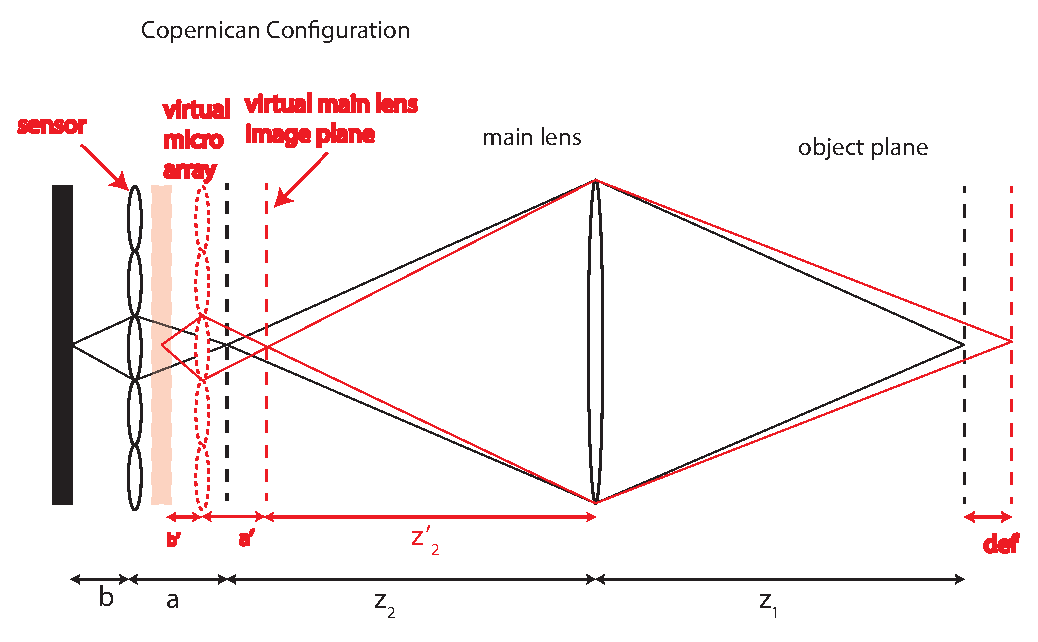
\includegraphics[width=1\textwidth]{C:/Users/Massimo/Documents/Thesis/ref20.eps}
	\caption{\label{fig:def20} The points that belong to out of focus object plane represented in red are imaged on a virtual main lens image plane. This plane is relayed on a virtual sensor plane by a virtual micro array whose parameters are  \textit{a'} and \textit{b'} and \textit{m' = b'/a'}. }
\end{figure}
The distance between the main lens image plane and the virtual main lens image plane, defined as \textit{$\bar{a} = a-a'$}, is called virtual depth \cite{perwass2012single}. The magnification of the virtual lenslet array defines the patch size to use to render the point at that particular depth. The link between the magnification \textit{m'} and \textit{m} can be defined by applying the lens law twice, once for the main lens and once for the micro array stage.
Therefore the virtual main lens plane corresponding to a defocus \textit{d} is located at:
\begin{equation}
	\label{eq:def201}
	z'_2 = \dfrac{(z_1+d)f}{(z_1+d)+f}
\end{equation}
where \textit{f} is the focal length of the main lens. The corresponding virtual depth value is given by subtracting the quantities $z'_2$ and $z_2$
\begin{equation}
\label{eq:def202}
\bar{a} = z'_2-z_2
\end{equation}
Then from the virtual depth $\bar{a}$ the values \textit{a'} and \textit{b'} for the virtual micro array can be obtained.
\begin{equation}
\begin{cases}
a' = a-\bar{a}   \\
b' = \dfrac{a'f}{a'+f} \\
\end{cases}
\end{equation}
And the magnification for the virtual plane is:
\begin{equation}
\label{eq:def204}
m' = \dfrac{b'}{a'}
\end{equation}
Values of the magnification $m'$ plotted as a function of defocus are shown in figure \ref{fig:def202}
\begin{figure}[H]
	\centering
	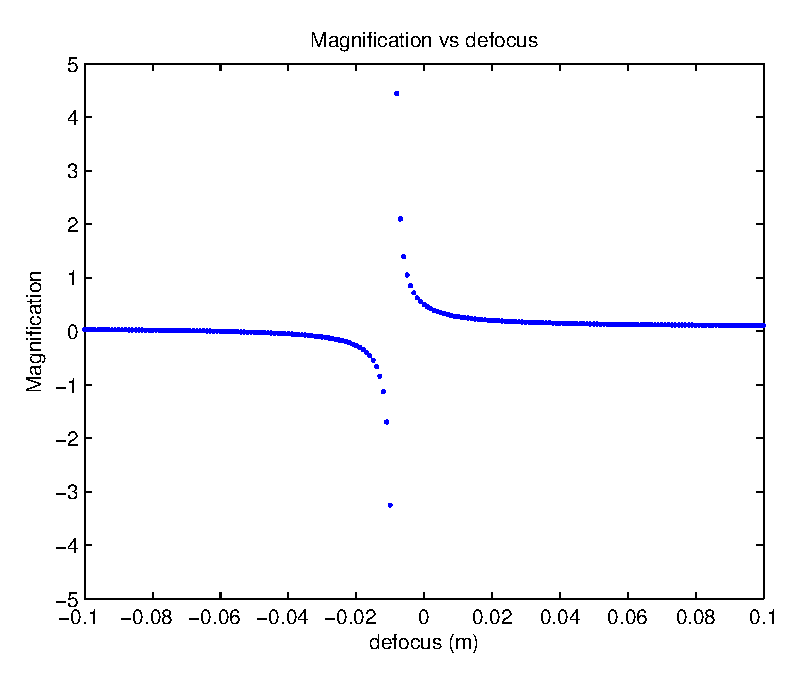
\includegraphics[width=.8\textwidth]{C:/Users/Massimo/Documents/Thesis/magn_def.eps}
	\caption{\label{fig:def202} Values of the magnification used to determine the patch size for the plenoptic 2.0 rendering plotted as a function of the defocus.  }
\end{figure}
The patch size corresponding to the new focal plane is therefore:
\begin{equation}
	\label{eq:patch2}
	\mu' = Pm' = P\dfrac{b'}{a'}
\end{equation}
Rendering with the new patch size allows refocusing at a different plane. If the defocus in not know, as in the majority of the cases, it is possible to estimate the depth information of the scene imaged and using this information to render the final image. These algorithms are based on cross correlating each sub image with its closest neighbours in order to evaluate the relative shift due to a change in depth across the lenslet\cite{hansen2011depth,johannsen2013calibration}. In this way it is possible to determine the patch size that results in the best match with all of its neighbours \cite{georgiev2010focused,lumsdaine2008full}.  \\
The axial resolution of a plenoptic 2.0 system is determined by considering that the minimum detectable shift between sub images formed by neighbouring lenslets is the one equal to one pixel. 
\section{Description of the system}
\label{sec:descrSYS20}
The system simulated is shown in figure \ref{fig:sys}. The main lens is in a 2f configuration, therefore $z_1$ = $z_2$ =\textit{z}.
\begin{figure}[H]
	\centering
	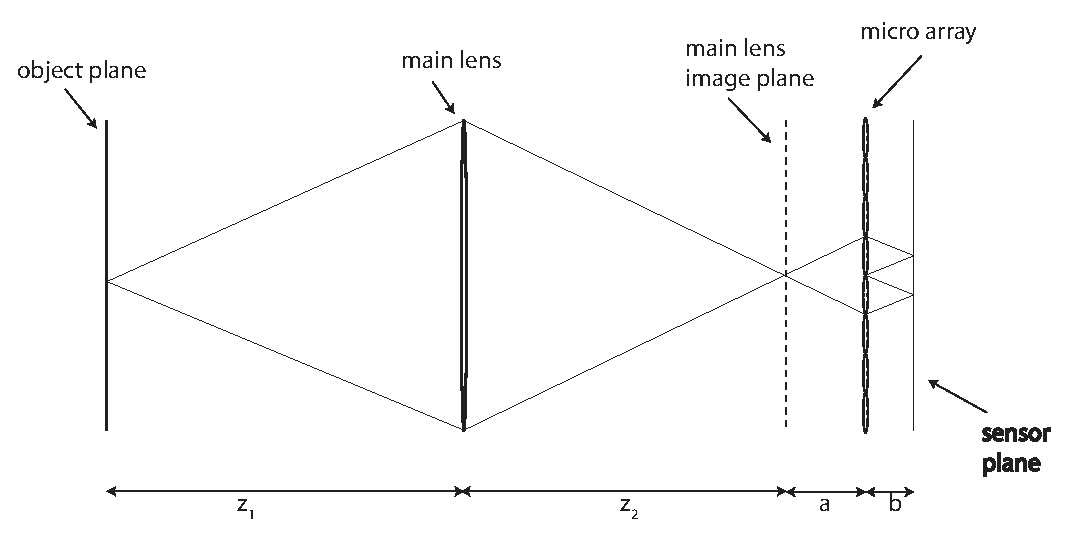
\includegraphics[width=.7\textwidth]{C:/Users/Massimo/Documents/Thesis/p20sys.eps}
	\caption{\label{fig:sys} Ray diagram of the system simulated.  }
\end{figure}
The main objective of the simulation on a plenoptic 2.0 system was to investigate its behaviour at the diffraction limit as well as to better understand the trade-offs in resolution and how the different parameters affect it. Different combinations of the optical parameters of the system, including main lens aperture, micro array pitch and magnification,  have been tested. The modularity of the Fresnel simulation toolbox allows to easily change the simulation parameters independently and collect results.
The system parameters are defined; these are the  dimension and the number of pixels on the sensor, the pitch and focal length of the lenslet array, the focal length of the main lens and the magnification $m$ of the micro array stage. The simulation toolbox is capable of automatically setting all other simulation parameters to respect the f-number matching between the main lens and the lenslet array. In a plenoptic 2.0 imaging system the f-number is matched when:
\begin{equation}
\label{eq:fmatch20}
\dfrac{z_2}{d}=\dfrac{b}{p}
\end{equation}
If the lenslet array has a focal length equal to $f_{\mu}$ and a pitch equal to \textit{p}, the value of the distance from the sensor \textit{b} can be obtained from the magnification \textit{m} as:
\begin{equation}
\label{eq:b}
b = mf_{\mu} \left(1+\dfrac{1}{m}\right)
\end{equation} 
Equation \ref{eq:b} has been obtained by substituting the expression of the magnification $m=b/a$ into the lens equation $1/a+1/b=1/f_{\mu}$.
Values of the parameter \textit{b} as a function of the magnification can be seen plotted in figure \ref{fig:b}
\begin{figure}[H]
	\centering
	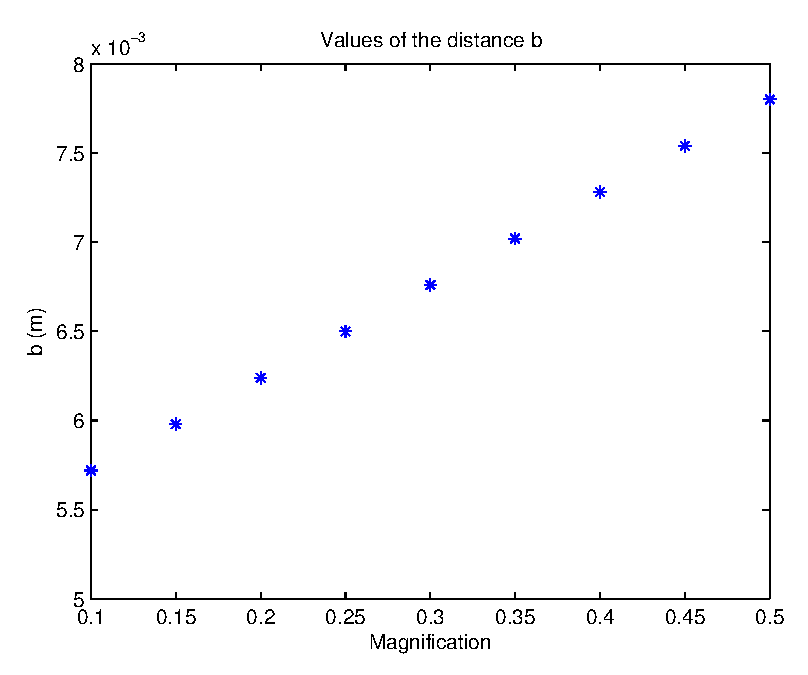
\includegraphics[width=.7\textwidth]{C:/Users/Massimo/Documents/Thesis/b.eps}
	\caption{\label{fig:b} Values of the parameter \textit{b} correspondent to values of magnification varying from 0.1 to 0.5.}
\end{figure}
\begin{figure}[H]
	\centering
	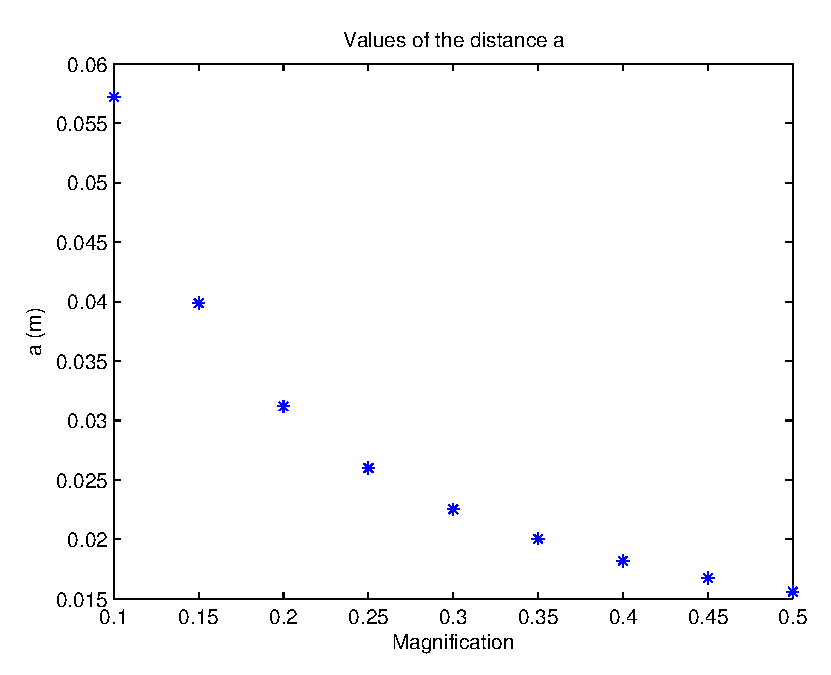
\includegraphics[width=.7\textwidth]{C:/Users/Massimo/Documents/Thesis/a.eps}
	\caption{\label{fig:a} Values of the parameter \textit{a} corresponding to values of magnification varying from 0.1 to 0.5.}
\end{figure}
Once \textit{b} is defined the distance of the micro lens array from the main lens image is calculated by solving the lens law for \textit{a}:
\begin{equation}
	\label{eq:a}
a = \dfrac{bf}{b-f}
\end{equation} 
Values of \textit{a} as a function of the magnification can be seen in figure \ref{fig:a}:
Now that the relay system has been defined, the software defines the aperture of the main lens matching its f-number to the one of the lenslet using equation \ref{eq:fmatch20}:
\begin{equation}
	\label{eq:radiuslens}
r_{lens} = \dfrac{zp}{2b}
\end{equation}
where $r_{lens}$ is the radius of the lens aperture.
Values of lens aperture radius as a function of the magnification can be seen in figure \ref{fig:aperture1}
\begin{figure}[H]
	\centering
	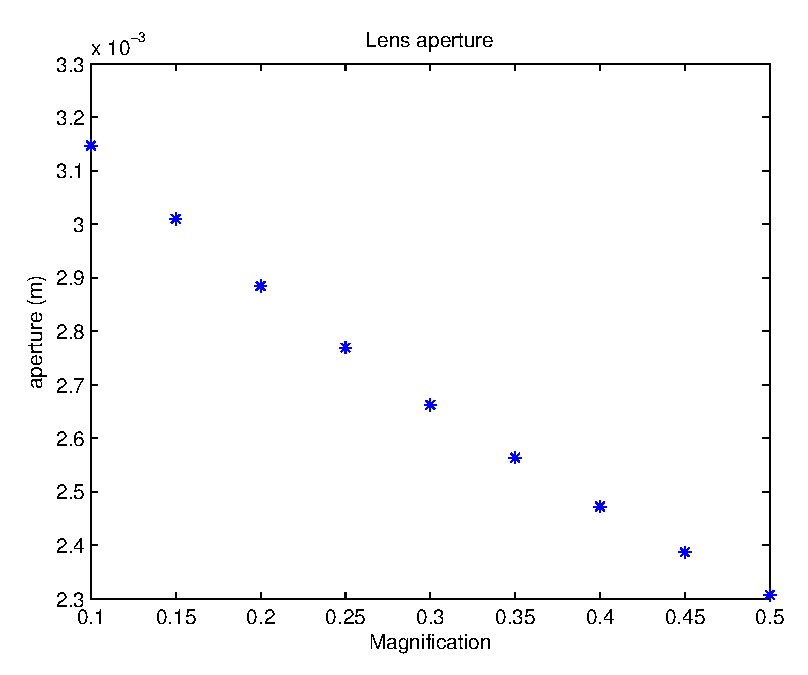
\includegraphics[width=.7\textwidth]{C:/Users/Massimo/Documents/Thesis/aperture.eps}
	\caption{\label{fig:aperture1} Aperture radius of the main lens as a function of the magnification in order to respect the f-number matching condition.}
\end{figure}
Therefore the simulation defined by the user, the remaining parameters are automatically set depending on the constraints discussed above, making the launching procedure of each simulation easy and quick.
The micro lens array is set with the following characteristics:\\
\\
\begin{center}
	\begin{tabular}{l|r}
	
		\centering
		Array size & 5.8 $\times$  5.8 mm\\ \hline
		Micro lens focal length $f_{\mu}$ & 5.3 mm \\ \hline
		Micro array pitch p & 150 $\mu m$ \\ \hline
		sensor size & 5.8 $\times$  5.8 mm\\ \hline
		sensor resolution & 3500 $\times$  3500 pixel \\ \hline
		pixel size & 1.67 $\mu m$ \\ \hline
		number of lenslet & 39 $\times$ 39  \\ \hline
		main lens focal length & 60 \textit{mm}
		\label{tab:4}
	\end{tabular}
\end{center}
And the values obtained for \textit{a,b} and the main lens aperture corresponding to the magnification investigated are:
\begin{center}
\begin{tabular}{l|c|c|r}
	\centering
	Magnification & \textit{a} & \textit{b} & main lens aperture\\ \hline
	0.5 & 15.6 \textit{mm} &  7.8 \textit{mm} & 2.3 \textit{mm}\\ \hline
    0.3 & 22.5 \textit{mm} &  6.8 \textit{mm} & 2.7 \textit{mm}\\ \hline
   	0.25 & 26.0 \textit{mm} &  6.5 \textit{mm} & 2.8 \textit{mm}\\ 
  	\label{tab:3}
\end{tabular}
\end{center}

\section{Optical Performances of a Focused Plenoptic System}
\label{sec:performances}
This section shows the results obtained running simulations of the system described is section \ref{sec:descrSYS20} at its diffraction limit. Three different configurations of the micro lens array stage have been tested, corresponding to the parameters \textit{a} and \textit{b} set in order to have magnification \textit{m = b/a} equal to 0.5, 0.3 and 0.25.
The first simulation presented is the image of a single focused point source. A comparison between the main lens image and the rendered image will be done to understand the differences in optical resolution and to evaluate the noise induced by the rendering algorithm.
The optical resolution of an imaging system is defined by its impulse response, known as point spread function \cite{goodman2005introduction,pedrotti1993introduction}. If the input is a point source in focus, the output image for an unaberrated circular aperture has a well known intensity profile, the Airy disk. The Airy disk defines the broadening that a point source undergo after being imaged by an optical system, hence it is a good estimation of the minimum feature resolvable by the system \cite{goodman2005introduction,herzig1997micro}. The Airy disk is shown in figure \ref{fig:airydisk}.  \\
The total extension of the central lobe is defined as the distance between the first two zeros as:
\begin{equation}
	\label{eq:airy3}
	\Delta x = 2.44 \lambda F_\# = 2.44 \lambda \dfrac{b}{p}
\end{equation}
The central lobe contains the $90 \%$ of the total energy of the optical field \cite{goodman2005introduction}, therefore its extension defines the spread that each point undergoes in the final image. 
\begin{figure}[H]
	\centering
	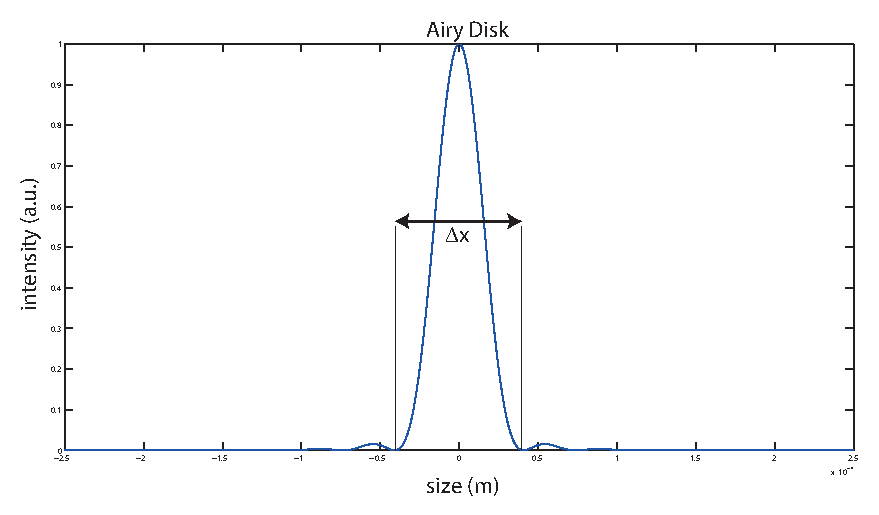
\includegraphics[width=.9\textwidth]{C:/Users/Massimo/Documents/Thesis/airydisk.eps}
	\caption{\label{fig:airydisk} Aperture of the main lens as a function of the magnification in order to respect the f-number matching condition.}
\end{figure}
$\Delta x$ is defined as the optical resolution of the imaging system.
In a plenoptic 2.0 system there are two elements that influence the optical resolution, the main lens and the micro lens array. Because of the f-number matching condition, the optical resolution in the two imaging stages should be the same. But because of the magnification present in the micro array stage, which is different from the magnification of the main lens, the coordinates in the main lens image plane are rescaled by a factor equal to the magnification \textit{m} when imaged by the micro array on the sensor \cite{goodman2005introduction}. Using the coordinates $x'$ and $y'$ of the main lens image plane, the sub image coordinates will be given by:
\begin{equation}
	\label{eq:rescale}
	\begin{cases}
		x = \dfrac{x'}{m}
		\\
		\\
		y = \dfrac{y'}{m}
	\end{cases}
\end{equation}   
Therefore if a pixel on the main lens image samples a feature size of $\delta x$, on the sensor the same pixel will sample a quantity $\delta x/m$. Because \textit{m} is smaller than 1, the spread of a point on the sensor plane will be bigger than the one on the main lens image plane. The same pixel samples a bigger area of the object in the image. This leads to a loss in optical resolution \cite{turola2014wave}. The smaller the magnification, the broader the point spread function and as a consequence the band pass of the micro lens array becomes narrower.
The optical cut off frequency is defined as:
\begin{equation}
	\label{eq:cutoff1}
	\nu_{cutoff} = m\dfrac{1}{\lambda f_\#} = m\dfrac{b}{\lambda p}
\end{equation}
Figure \ref{fig:lateral} shows the values of the lateral resolution plotted as a function of the magnification of the micro array stage, while figure \ref{fig:freq} shows the correspondent values of the optical cut off frequency.
\begin{figure}[H]
	\centering
	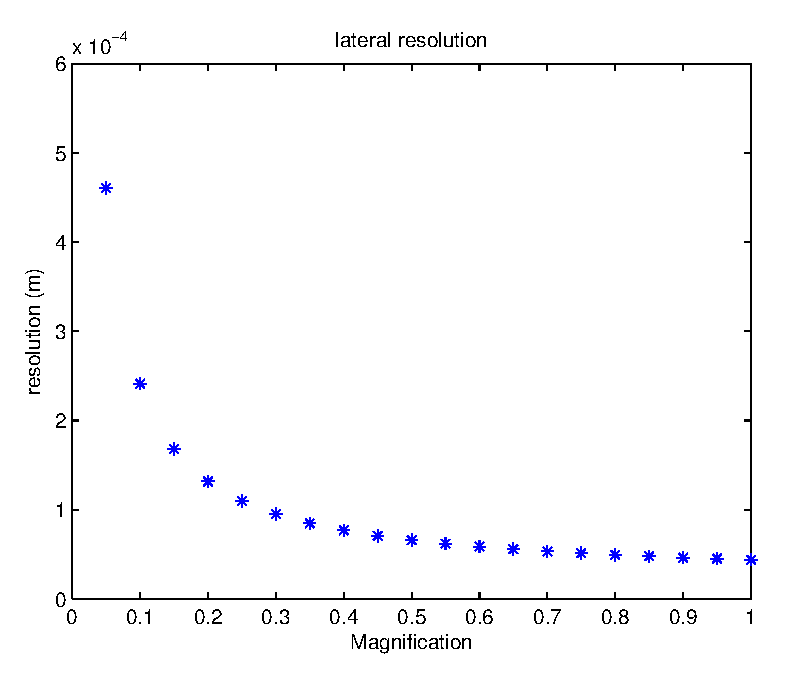
\includegraphics[width=.7\textwidth]{C:/Users/Massimo/Documents/Thesis/res.eps}
	\caption{\label{fig:lateral} Lateral resolution as a function of the magnification.}
\end{figure}
\begin{figure}[H]
	\centering
	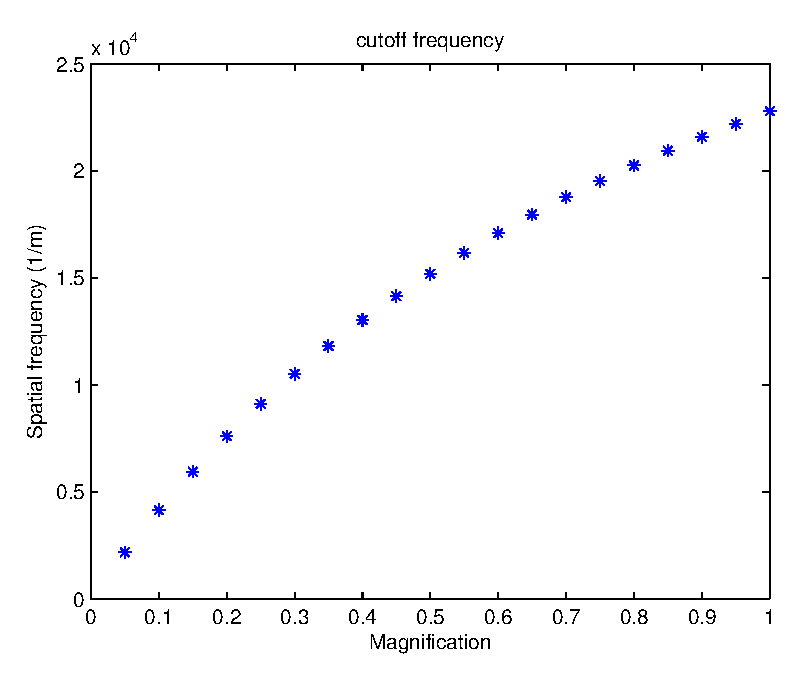
\includegraphics[width=.7\textwidth]{C:/Users/Massimo/Documents/Thesis/spatial.eps}
	\caption{\label{fig:freq} Optical cut-off frequency as a function of the magnification.}
\end{figure}
This means that in a plenoptic 2.0 imaging system there is an intrinsic trade-off between optical resolution and spatio-angular resolution. The trade off between spatial and angular resolution has been described in section \ref{sec:pleno20}. A further trade off is now present and it is due to diffraction. A low magnification enables good sampling of the direction and therefore a finer axial resolution when evaluating depth, but a magnification that is too low will filter out high frequency components of the object. \\
The next sections will investigate in detail the optical performances of a focused plenoptic system, performing simulations to better understand the trade off between spatio-angular resolution and optical resolution. This is the first study in plenoptic research whose goal is to evaluate the effects of the optical parameters of a focused plenoptic system on its optical resolution using a wave optics approach.
\section{Impulse Response of a Focused Plenoptic system}
\label{sec:impulse}
The first simulation performed was designed to obtain the impulse response of a focused plenoptic system. The point source has been simulated using a pupil with a diameter of 10 $\mu m$.\\
As explained in section \ref{sec:rendering}, the magnification of the lenslet array gives the number of points of view that sample an image. To have directional information, a point of the object should be sampled at least by two points of view, therefore by two  lenslets. In this way two sets of directional coordinates are captured on the sensor and each point is repeated four times in the raw image, twice horizontally and twice vertically.This is the case for a magnification of 0.5. With a magnification of 0.3 each point is expected to be replicated 3 times, and with a magnification of 0.25 four times.\\
Figures \ref{fig:point05}, \ref{fig:point03}, and \ref{fig:point025} show the raw sensor images and the rendered images of a point source when the magnification is 0.5, 0.3 and 0.25.  
\begin{figure}[H]
	\centering
	
\includegraphics[width=1\textwidth]{C:/Users/Massimo/Documents/Thesis/raw05.eps}
	\caption{\label{fig:point05} Left: raw sensor image of a point source, Right: rendered image. Artifacts are present. Magnification of the lenslet array: 0.5 }
\end{figure}
\begin{figure}[H]
	\centering
	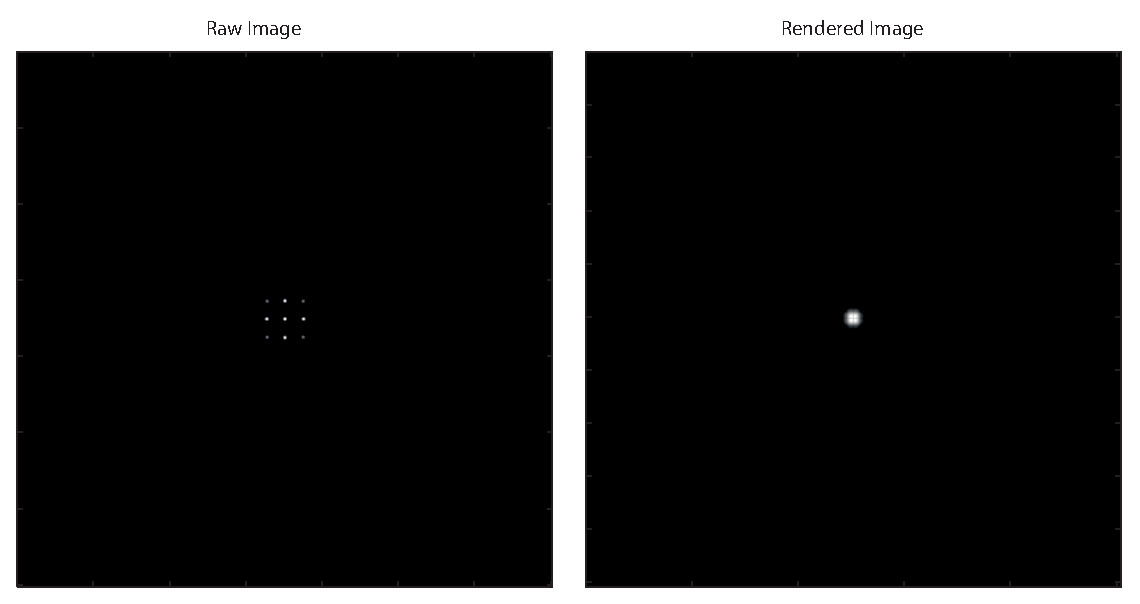
\includegraphics[width=1\textwidth]{C:/Users/Massimo/Documents/Thesis/raw03.eps}
	\caption{\label{fig:point03} Left: raw sensor image of a point source, Right: rendered image. Artifacts are present. Magnification of the lenslet array: 0.3.}
\end{figure}
\begin{figure}[H]
	\centering
	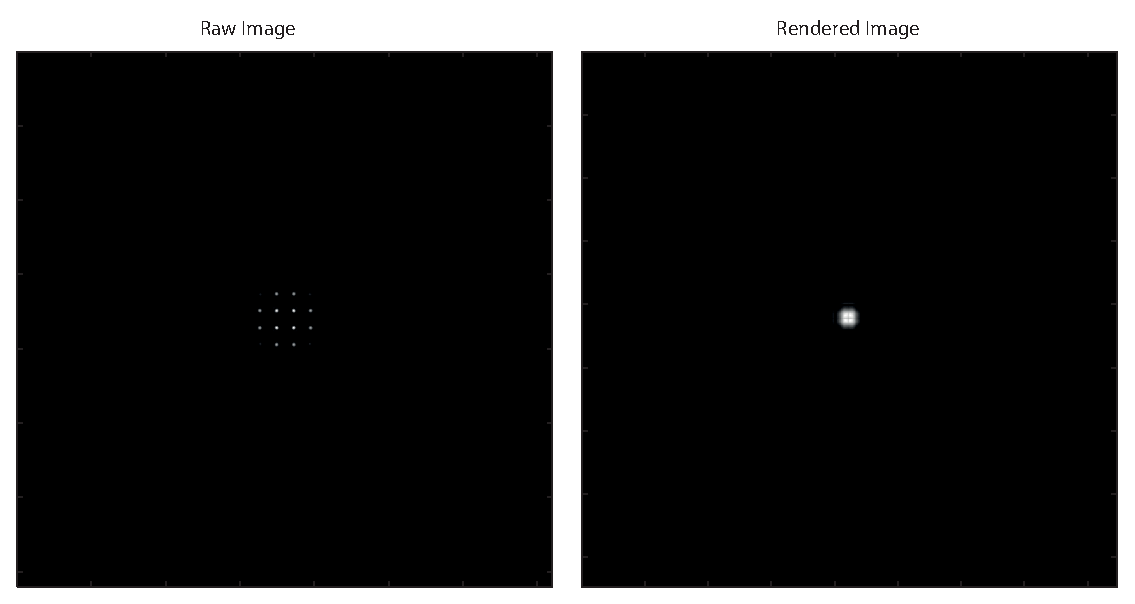
\includegraphics[width=1\textwidth]{C:/Users/Massimo/Documents/Thesis/raw025.eps}.
	\caption{\label{fig:point025} Left: raw sensor image of a point source, Right: rendered image. Artefacts are present. Magnification of the lenslet array: 0.25 }
\end{figure}
From figure \ref{fig:prof05} it is possible to appreciate the broadening effects of the central lobe of the rendered image intensity profile, in red, with respect to the main lens image. The central lobe size is also dependent on the magnification used as seen in figure \ref{fig:lateral}. With a small magnification, the number of sub images that sample a single point source increase, and due to the nature of the rendering process explained in section \ref{sec:basicrendering}, the number of artefacts increases, broadening the central lobe and making the lateral resolution worse.
\begin{center}
\begin{tabular}{l|c|c|r}
\centering
Magnification & $\Delta x$ (m)& $\Delta x'$ (m) & $\Delta x/\Delta x'$\\ \hline
0.5 & $7.848 \times 10^{-5}$ &  $2.000 \times 10^{-4}$ & 0.39\\ \hline
0.3 & $6.848 \times 10^{-5}$ &  $2.698 \times 10^{-4}$ & 0.25 \\ \hline
0.25 & $6.514\times 10^{-5}$ &  $3.574 \times 10^{-4}$ & 0.18 \\ 
\label{tab:5}
\end{tabular}
\end{center} 
Table \ref{tab:5} shows the values of the central lobe size of the main lens image, $\Delta x$, of the rendered image $\Delta x'$ and the ratio between them. The error in the ratio is due to the presence of artefacts generated by the rendering algorithm that increases with the decrease of the magnification.
\begin{figure}[H]
	\centering
	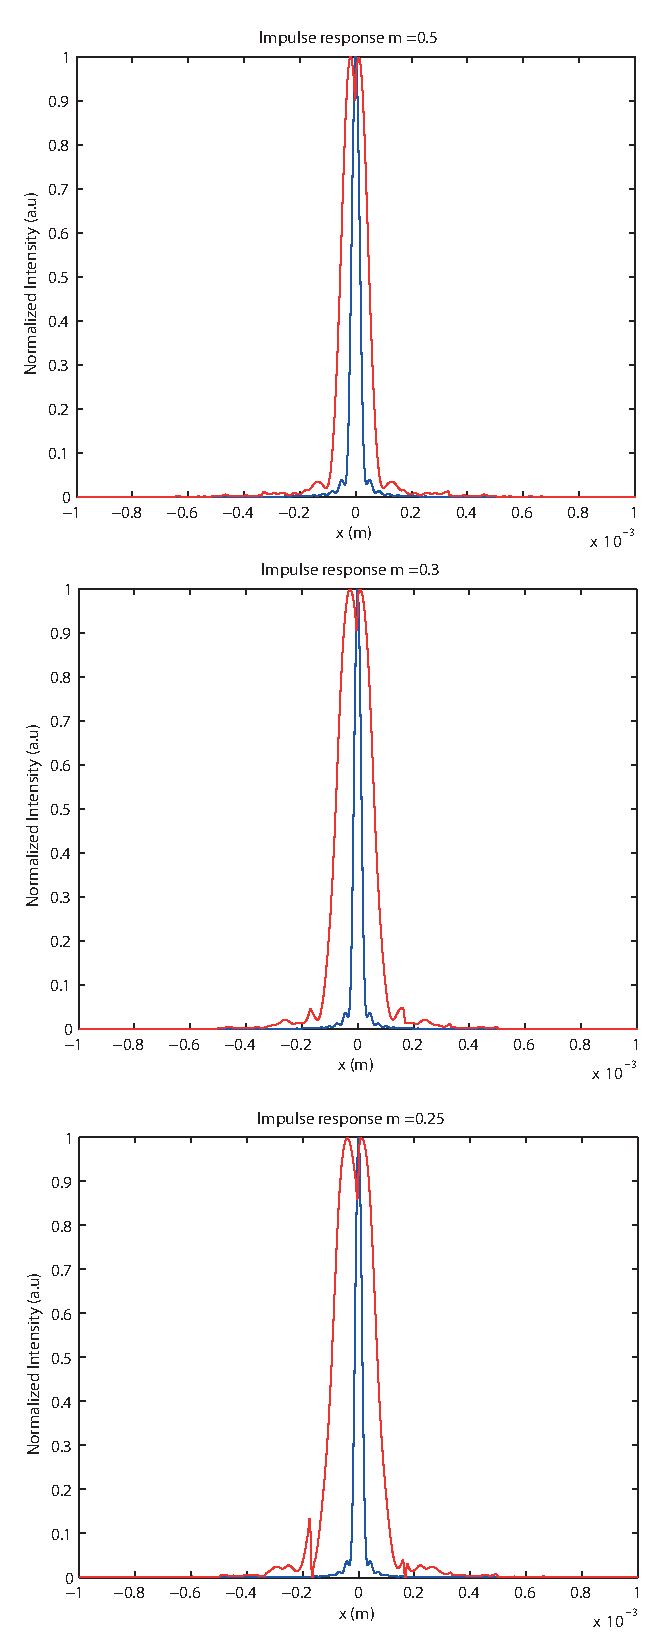
\includegraphics[width=0.45\textwidth]{C:/Users/Massimo/Documents/Thesis/crossect.eps}.
	\caption{\label{fig:prof05} From top to bottom: comparison between the main lens image profile, in blue, and the rendered image profile, in red, for magnification values of 0.5, 0.3 and 0.25. The central lobe of the rendered image increase with the magnification, as well as the number of artefacts. }
\end{figure}
\section{Two Point Resolution}
\label{sec:two}
Another important instrument to evaluate the resolution of an imaging system is the Rayleigh criterion of resolution. It states that two point sources whit a phase difference of $\pi/2$ imaged coherently  are resolved by a diffraction limited imaging system when the centre of the Airy disk intensity pattern generated by one point source falls exactly on the first zero of the Airy disk generated by the other point source \cite{goodman2005introduction}. The Rayleigh criterion of resolution states that for two point sources of light the minimum distance to resolve them both in the image plane is given  by:
\begin{equation}
	\label{eq:rayleigh}
	\delta x = 1.22\lambda\dfrac{z}{d}
\end{equation}
Where \textit{d} is the lens aperture and \textit{z} is the propagation distance.
In the simulation the two point sources were placed at distance equal to the Rayleigh distance and they have been imaged by a plenoptic 2.0 system where the micro lens array had a magnification of 0.5. The purpose of this experiment is to prove that the magnification of the micro lenses limits the optical resolution of the system. 
Figure \ref{fig:twopoint1} shows the main lens image and the rendered image with their respective intensity profiles, of two point source with a diameter of 10 $\mu m$ separated by a distance $\delta x = 40 \mu m$. The imaging system simulated is the same described in section \ref{sec:descrSYS20}.
While in the main lens image the two point sources are at the limit of resolution and the two points are still resolvable, in the rendered image the two spot sizes are merged together and no longer resolvable.
\begin{figure}[H]
	\centering
	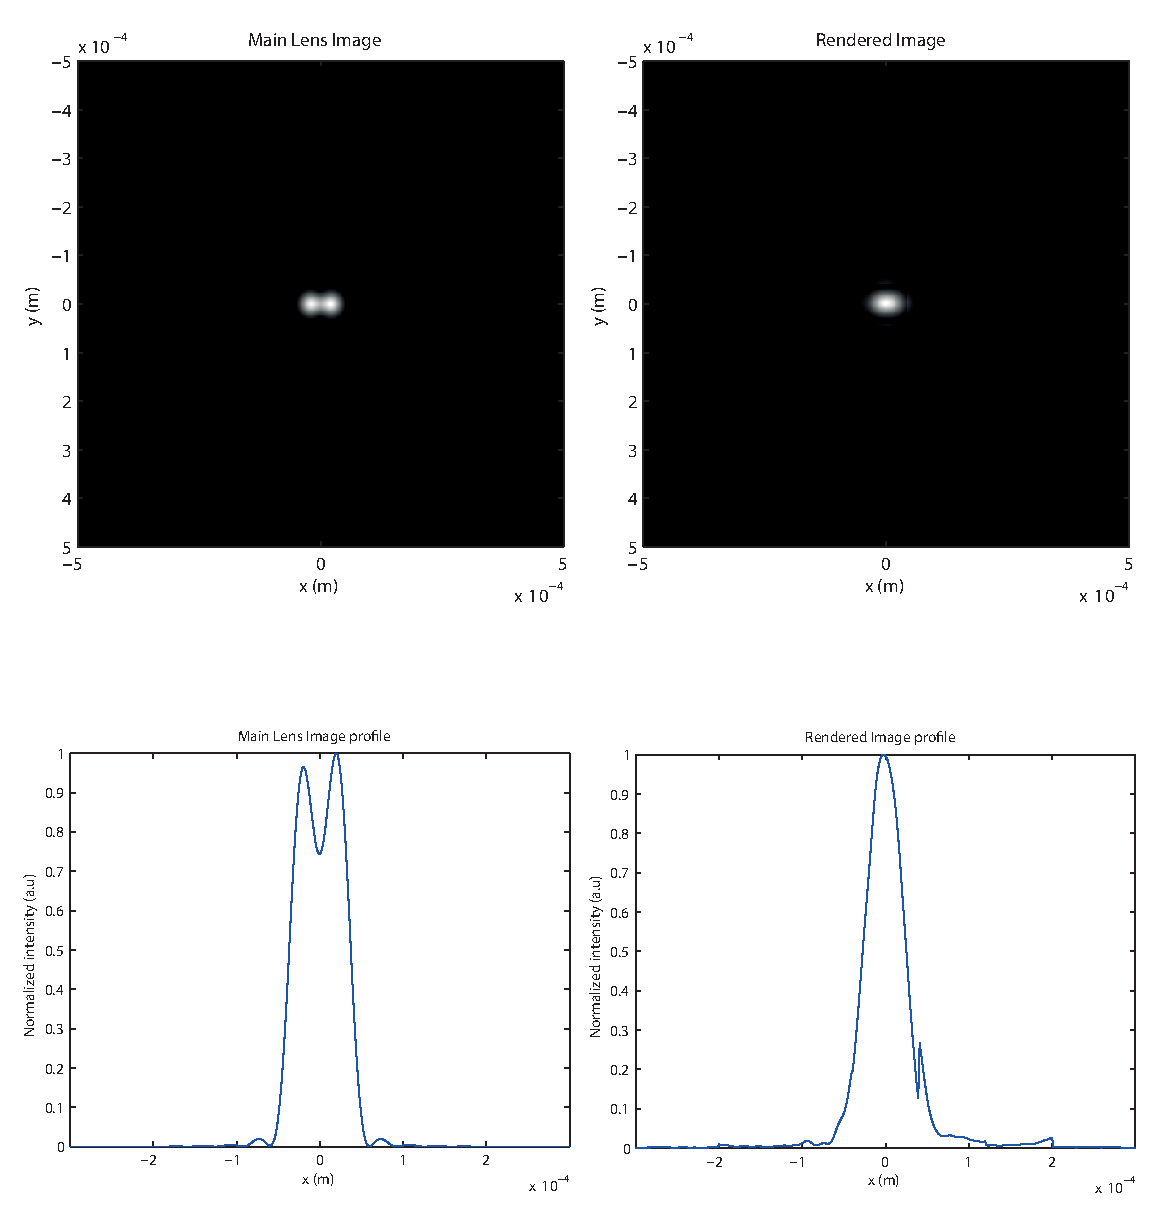
\includegraphics[width=1\textwidth]{C:/Users/Massimo/Documents/Thesis/two_points.eps}.
	\caption{\label{fig:twopoint1} On the top left there is the main lens image of two point sources separated by the Rayleigh distance $\delta x$. On the top right its corresponding rendered plenoptic image obtained with a magnification of 0.5. As expected from the theory, the resolution of the rendered image is half the one af the main lens image, and the two points are no more distinguishable as confirmed by the intensity profiles of the two images on the bottom.   }
\end{figure}
If the separation between the point sources is doubled in the object plane they should be resolved in the rendered image too while keeping the magnification 0.5. Figure \ref{fig:twopoint2} shows the simulations results for a $\delta x = 80 \mu m$:
\begin{figure}[H]
	\centering
	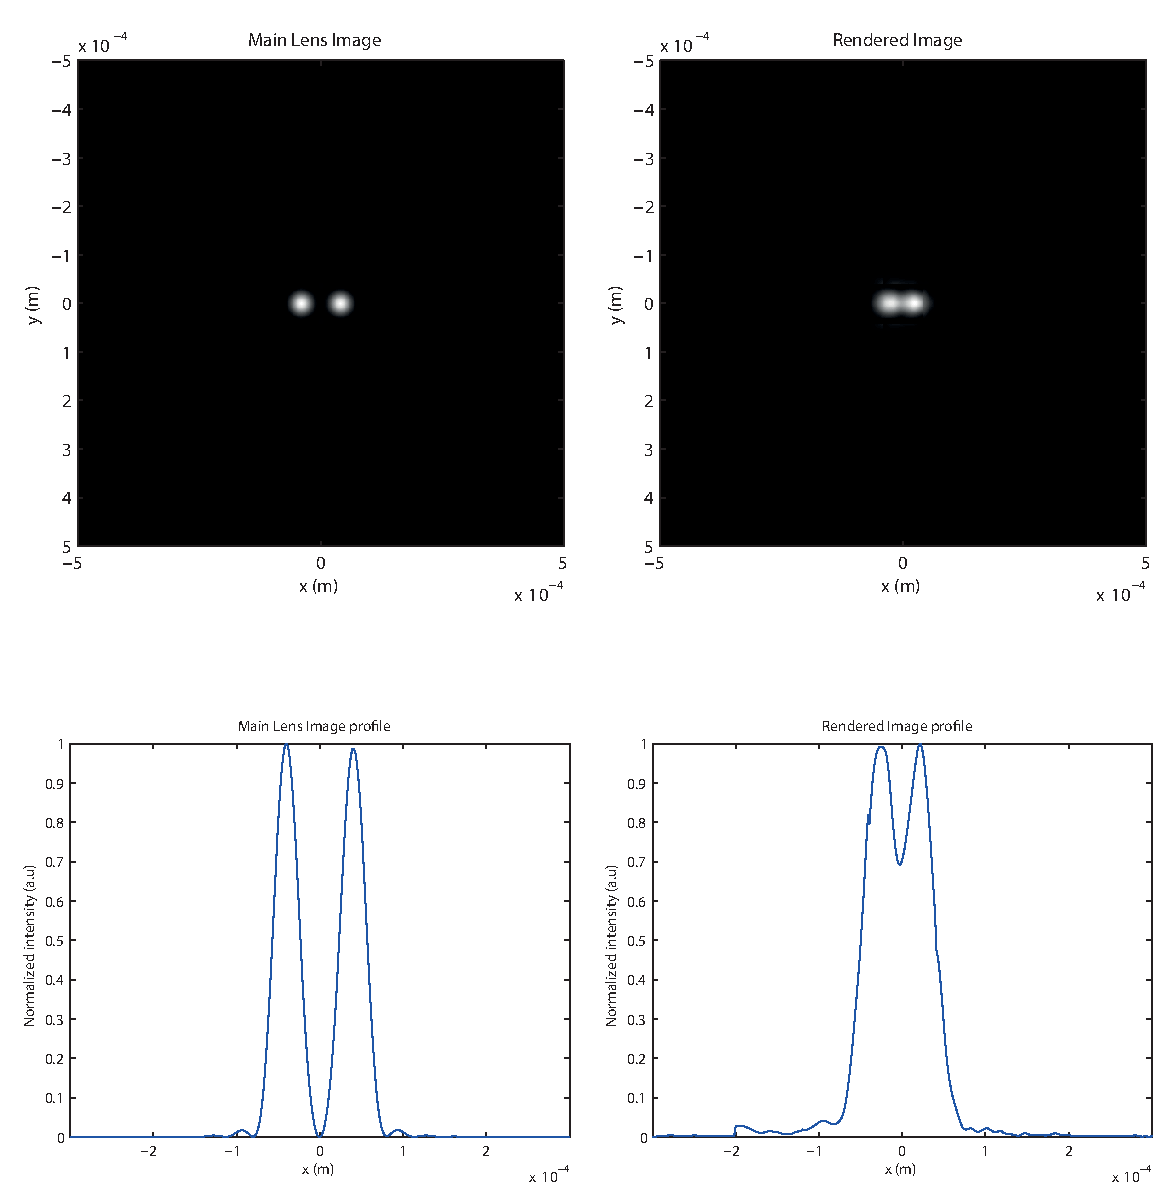
\includegraphics[width=1\textwidth]{C:/Users/Massimo/Documents/Thesis/twopoints2.eps}.
	\caption{\label{fig:twopoint2} The image on the top left shows  the main lens image of two point sources separated by the Rayleigh distance $2\delta x$. On the top right there is its corresponding rendered plenoptic image obtained with a magnification of 0.5. Doubling the Rayleigh distance the rendered image is at the limit of resolution, where the maximum of the Airy pattern of one point falls on the first zero of the second point. }
\end{figure}
These results obtained by simulating wave optics propagation in the plenoptic imaging system confirm the predictions made in section \ref{sec:performances} and it is the first experiment of this kind. When imaging an object with a plenoptic 2.0 system the loss of resolution due to the magnification should be taken into account in order not to lose useful information in the sample, or a suitable lenslet array configuration should be chosen.
\section{Frequency Analysis of a Focused Plenoptic System}
\label{sec:freq}
This section will describe the frequency response of a focused plenoptic system and its dependency on the magnification of the lenslet array stage. The spatial frequencies that are transferred from the object to the image plane in an optical system are defined by its modulation transfer function (MTF). The MTF is defined as the square modulus of the Fourier transform of the impulse response \textit{h(x,y)} of an optical system \cite{goodman2005introduction}. \\
It is then:
\begin{equation}
	\label{eq:OTF}
	H(f_x,f_y) = |\mathcal{F}\{h(x,y)\}|
\end{equation}
It represents the weighting factor applied by the system to all the frequency components of the optical field coming form the object. The visibility and the contrast of the points corresponding to the different values of spatial frequency changes according to the modulation imposed by the MTF. When it goes to zero, no energy is transmitted for that particular frequency and the detail is no longer present in the image.
The value of spatial frequency  for which the MTF goes to zero is called optical cut-off frequency. In this section the effects of the magnification on the location of optical cut-off frequency is investigated. The first result presented is obtained by calculating the modulation transfer function of the plenoptic 2.0 system described in section \ref{sec:impulse}, with magnification values of 0.5, 0.3 and 0.25. The MTF for these three cases are shown in figure \ref{fig:MTF} and have been obtained applying equation \ref{eq:OTF} to the intensity profiles in figure \ref{fig:prof05}. In all the three figures in green is represented the MTF of the single lens imaging system, without the lenslet array stage, and in red is represented the MTF of the plenoptic system.\\
From figure \ref{fig:MTF} it is possible to see that the cut off frequency of the single lens system increases with the decreasing of the magnification, while the cut-off frequency decrease with the decreasing of the magnification if the lenslet array stage is added. This result is in accord with what seen in sections \ref{sec:performances} and is coherent with the simulations results shown in section \ref{sec:impulse}. The magnification of the micro lens array reduces the optical resolution. This is a direct consequence of the intrinsic trade-of between optical resolution and the spatio-angular resolution. While reducing the magnification of the micro array stage increases the number of directional samples, at the same time makes the optical bandwidth narrower, reducing the lateral resolution. The decrease in the optical cut-off frequency is directly proportional to the decrease of the magnification as predicted in the theory with equation \ref{eq:cutoff1} and proved by the numerical simulation. 
The values of the cut-off frequencies obtained by the simulations are:
\begin{center}
	\begin{tabular}{l|c|r}
		Magnification & Rendered $f_{cut-off}m^{-1}$ & Main lens $f_{cut-off}m^{-1}$\\ \hline
		0.5 & $1.00 \times 10^{4}$ &  $3.00 \times 10^{4}$ \\ \hline
		0.3 & $0.76 \times 10^{4}$ &  $3.50 \times 10^{4}$ \\ \hline
		0.25 & $0.63\times 10^{4}$ &  $3.60\times 10^{4}$  \\ 
		\label{tab:6}
	\end{tabular}
\end{center} 
\begin{figure}[H]
	\centering
	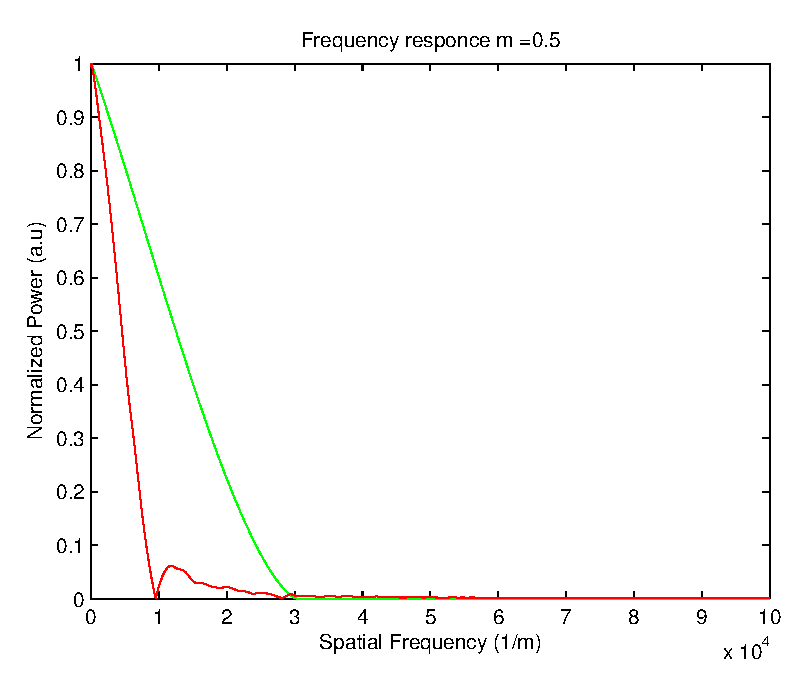
\includegraphics[width=0.5\textwidth]{C:/Users/Massimo/Documents/Thesis/MTF05.eps}.
	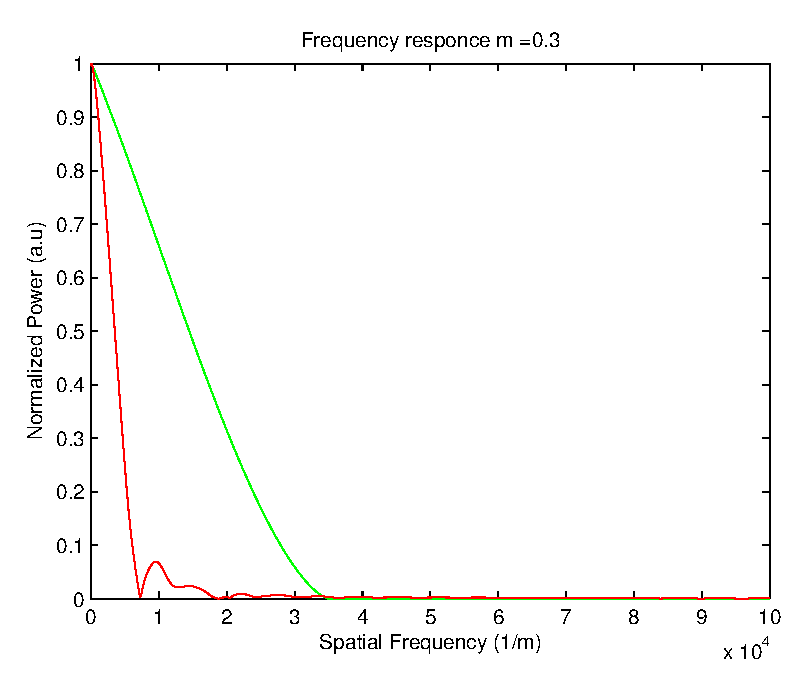
\includegraphics[width=0.5\textwidth]{C:/Users/Massimo/Documents/Thesis/MTF03.eps}.
	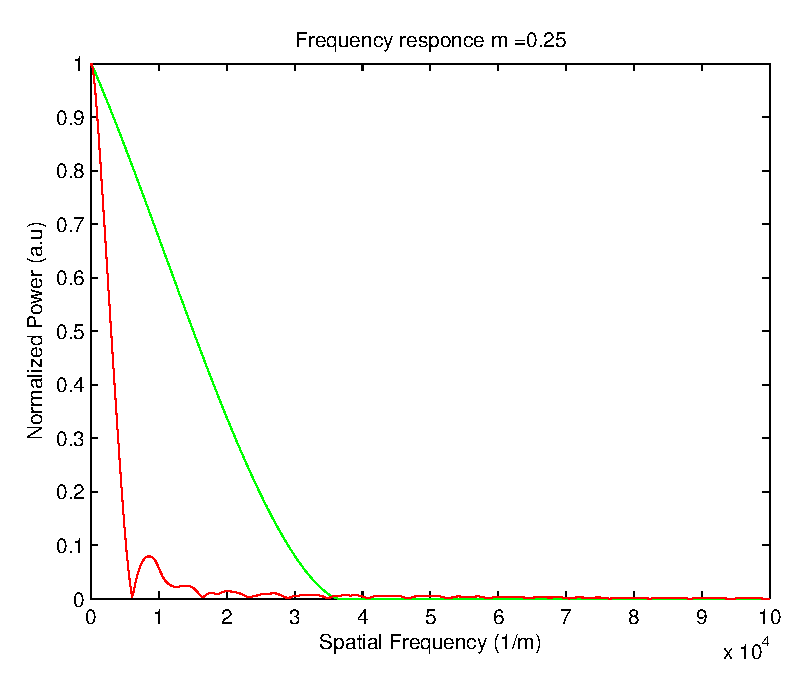
\includegraphics[width=0.5\textwidth]{C:/Users/Massimo/Documents/Thesis/MTF025.eps}.
	\caption{\label{fig:MTF} Modulation transfer functions of the main lens (green) and the overall imaging system (red) for a magnification value of \textit{m = 0.5} , top, \textit{m = 0.3}, central, and \textit{m = 0.25}, bottom.}
\end{figure}
The second set of simulations done evaluates the effects of the magnification in more detail. A varying frequency sinusoidal grating is imaged incoherently, as explained in chapter \ref{chap:fresnel}, by the system with the same three different configurations of the micro array stage. The grating contains five different frequencies :
\begin{center}
\begin{tabular}{l|r}
	\centering
	$f_1$ & $0.10\times 10^4 m^{-1}$ \\
	$f_2$ & $0.80\times 10^4 m^{-1}$ \\
	$f_3$ & $1.52\times 10^4 m^{-1}$ \\
	$f_4$ & $2.22\times 10^4 m^{-1}$ \\
	$f_5$ & $2.94\times 10^4 m^{-1}$ \\
\end{tabular}
\end{center}
\begin{figure}[H]
	\centering
	\includegraphics[width=0.7\textwidth]{C:/Users/Massimo/Documents/Thesis/pattern.eps}.
	\caption{\label{fig:pattern} The object imaged in this simulation is a sinusoidal grating containing five different frequencies. }
\end{figure}
Figure \ref{fig:image05} shows the raw image, the main lens image and rendered images of the sinusoidal grating shown in figure \ref{fig:pattern}, imaged with a magnification of \textit{m = 0.5}. The two rendered images are obtained with the basic rendering explained in section \ref{sec:rendering}. To remove digital artefacts given by the tiling of the sub images patches on the rendered images a low pass Gaussian filter with $\sigma = 1.162\times 10^4 $ has been applied.   
\begin{figure}[H]
	\centering
	\includegraphics[width=0.8\textwidth]{C:/Users/Massimo/Documents/Thesis/images05.eps}.
	\caption{\label{fig:image05} Top: on the left is the raw sensor image, on the right the main lens image. Bottom: On the left there is the  rendered image, on the right the same image has been low pass filtered to remove some of the rendering artefacts. Magnification was 0.5   }
\end{figure}
\begin{figure}[H]
	\centering
	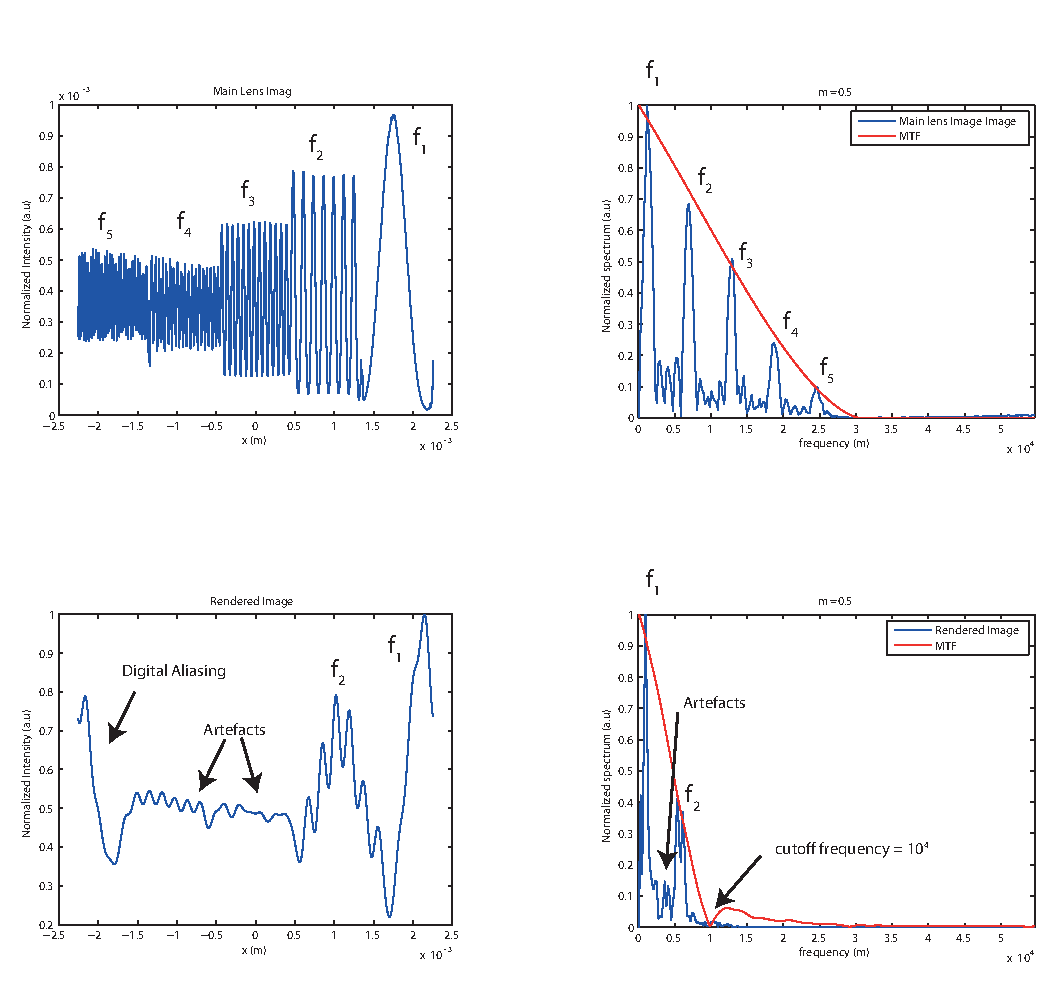
\includegraphics[width=1\textwidth]{C:/Users/Massimo/Documents/Thesis/MTF05final2.eps}.
	\caption{\label{fig:freq05}  On the left: intensity profiles of the main lens image, top and of the rendered image,bottom. On the right the spatial frequencies modulated according to the MTF as shown by the power spectra of the main lens image on the top right and of the rendered image on the bottom right. The magnification of the lenslet array is \textit{m = 0,5} and  the first zero frequency of the system is $f_{cut-off} = 10^4 m{-1}$}
\end{figure}
The normalized intensity profile of the optical field at the main lens image plane compared with the intensity profile of the rendered image is shown in figure \ref{fig:freq05}  on the left side while on the right the power spectra of the main lens image and of the rendered image is presented. The modulation transfer function of the main lens and of the full plenoptic system has been added in red.  \\
As expected the amplitude of the oscillations in both the main lens image and the rendered image follow the profile of the modulation transfer function of the two stages.  \\
Not all the frequency components of the object field are transmitted through the different stages of the plenoptic imaging system. In fact it acts as a low pass filter, whose bandwidth depends on the magnification used in the lenslet array stage. The low pass filtering action is shown in figure \ref{fig:block}.
\\
  It is interesting to see also that the rendered image presents some artefacts which are responsible for some extra frequencies present in the spectrum of the output rendered image. The cut off frequency of the imaging system with a magnification equal to 0.5 is $10^4 1/m$ therefore only the first two frequencies will be transmitted to the rendered image, as shown in figure \ref{fig:freq05}.
    If the magnification drops to \textit{m = 0.3} the bandwidth of the system gets narrower, and fewer frequencies are transmitted in the rendered image.
    \\
    Figure \ref{fig:image03} shows the raw image, the main lens image and rendered images of the sinusoidal grating shown in figure \ref{fig:pattern}
  \begin{figure}[H]
  	\centering
  	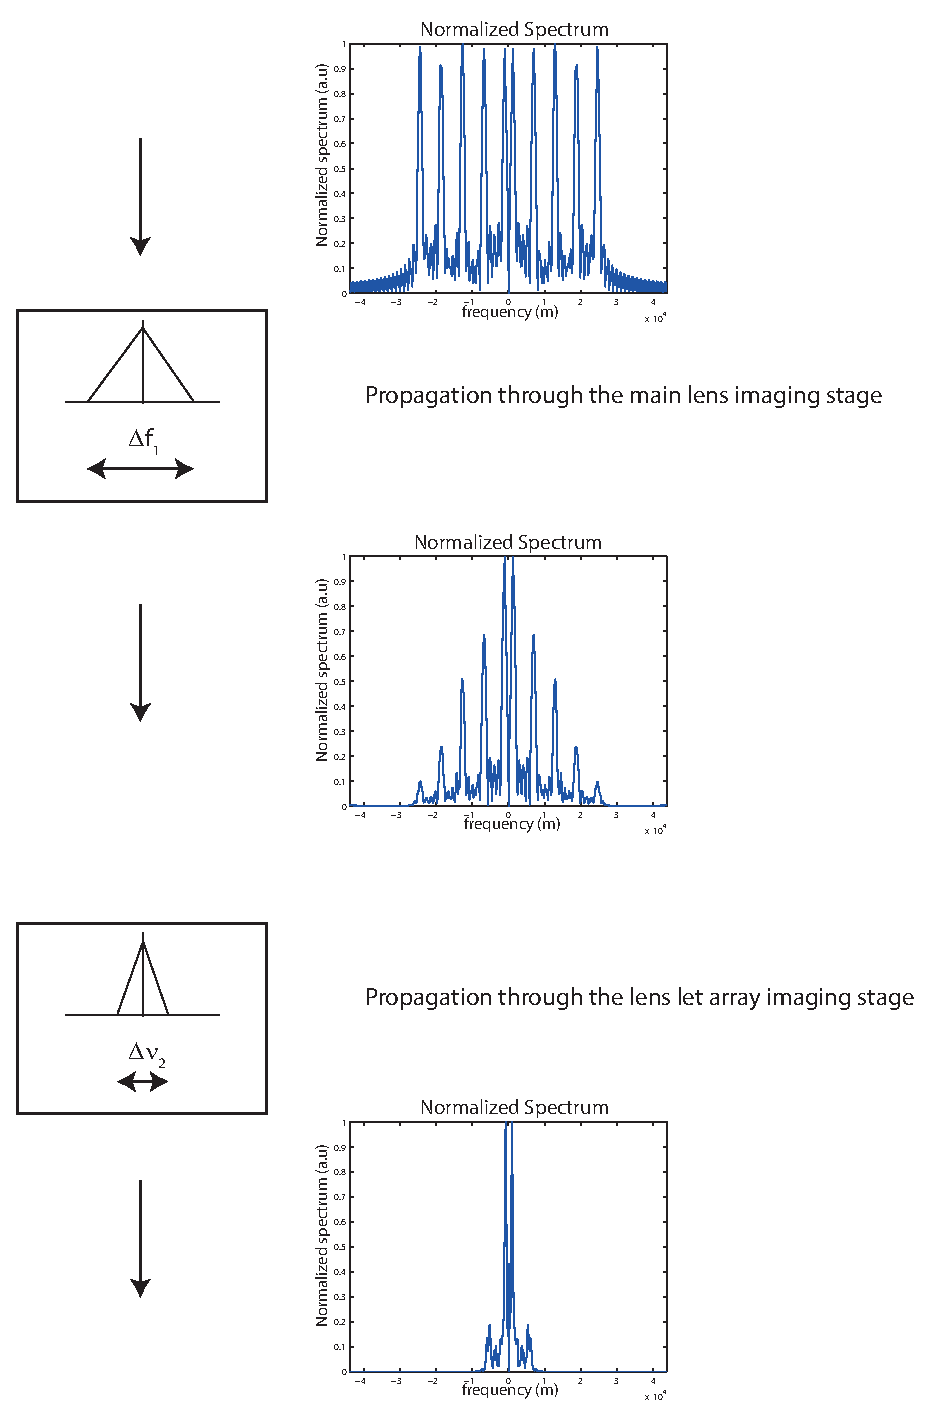
\includegraphics[width=.8\textwidth]{C:/Users/Massimo/Documents/Thesis/blockdiagram.eps}.
  	\caption{\label{fig:block} Evolution of the spectrum of the optical field as it propagates through the imaging system. First step the field is propagated through the main lens and its frequency content is modulated by its MTF whose bandwidth is $\Delta \nu_1$. Then modulated field passes through the lenslet array stage and because of the magnification that is less than zero its bandwidth is reduced further to $\Delta \nu_2$. Since $\nu_1 > \nu_2$  the imaging system is modelled as a linear low pass filter with a bandwidth $\Delta \nu_1$ defined by the magnification of the micro array stage. }
  \end{figure}
 \begin{figure}[H]
 	\centering
 	\includegraphics[width=1\textwidth]{C:/Users/Massimo/Documents/Thesis/MLI03SIN.eps}.
 	\caption{\label{fig:image03} Top: on the left it is shown the raw sensor image, on the right the main lens image. Bottom: On the left there is the  rendered image, on the right the same image has been low pass filtered to remove some of the rendering artefacts. Magnification was 0.3. }
 \end{figure}
As for the previous case figure \ref{fig:freq03} shows a comparison of the intensity profile of the main lens image with the rendered image one and of their respective power spectra: 
 \begin{figure}[H]
 	\centering
 	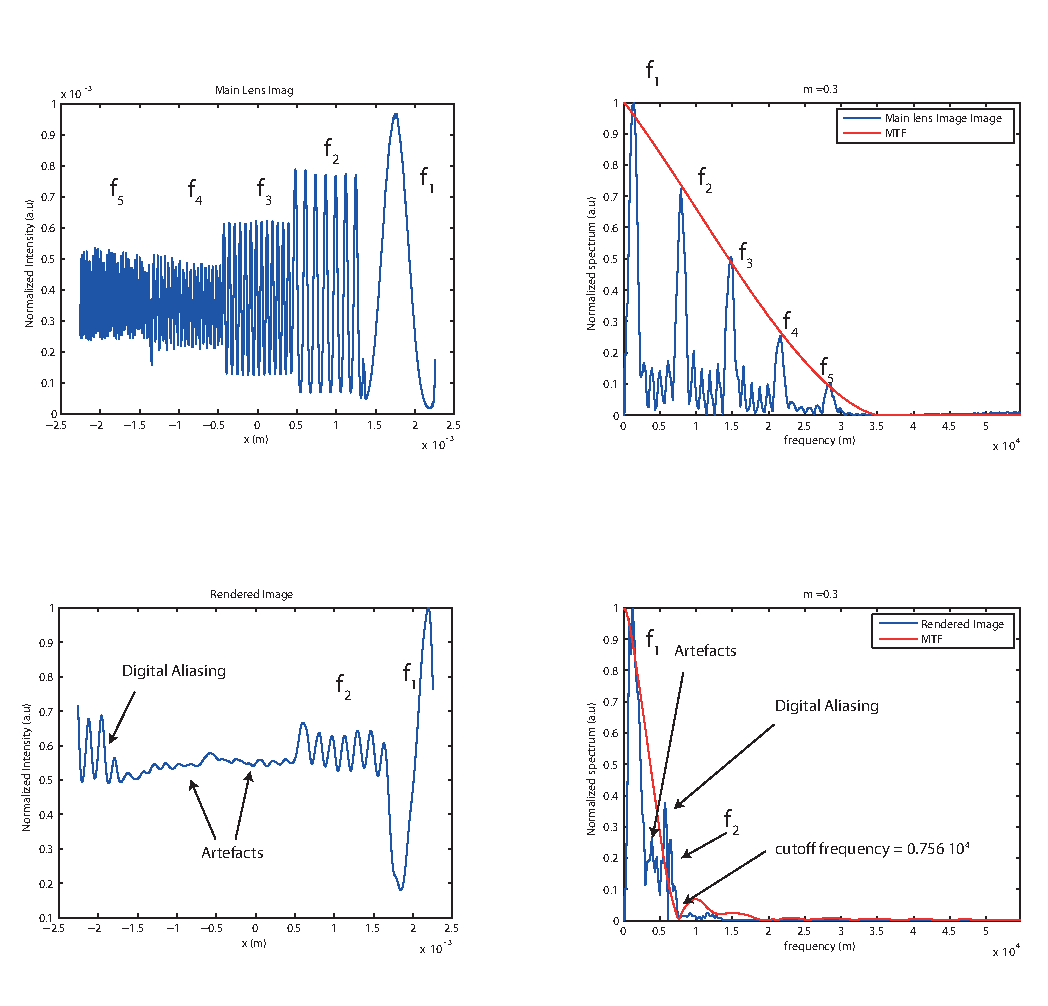
\includegraphics[width=1\textwidth]{C:/Users/Massimo/Documents/Thesis/MTF03final2.eps}.
 	\caption{\label{fig:freq03} On the left: intensity profiles of the main lens image, top and of the rendered image,bottom.On the right: spatial frequency modulation done by MTF. The first zero frequency of the system is $0.756 \times 10^4 m{-1}$}
 \end{figure}
 Figure \ref{fig:freq03} shows that the frequency $f_2$ gets attenuated more with respect to the previous case because it is closer to the first zero frequency of the system. The spectrum of the rendered image allows to discriminate between frequencies due to artefacts and digital aliasing in the rendering process. Their frequency is smaller than the one predicted by the modulation transfer function for that location in the rendered image. These frequencies are indicated in figure \ref{fig:freq03} with an arrow as artefacts. Low frequencies components generated by digital aliasing in the main lens image, have been picked up by the micro array relay stage and transmitted to the rendered image as indicated in figure \ref{fig:freq03}. These effects can be seen in detail in figure \ref{fig:aliasing}:
 \begin{figure}[H]
 	\centering
 	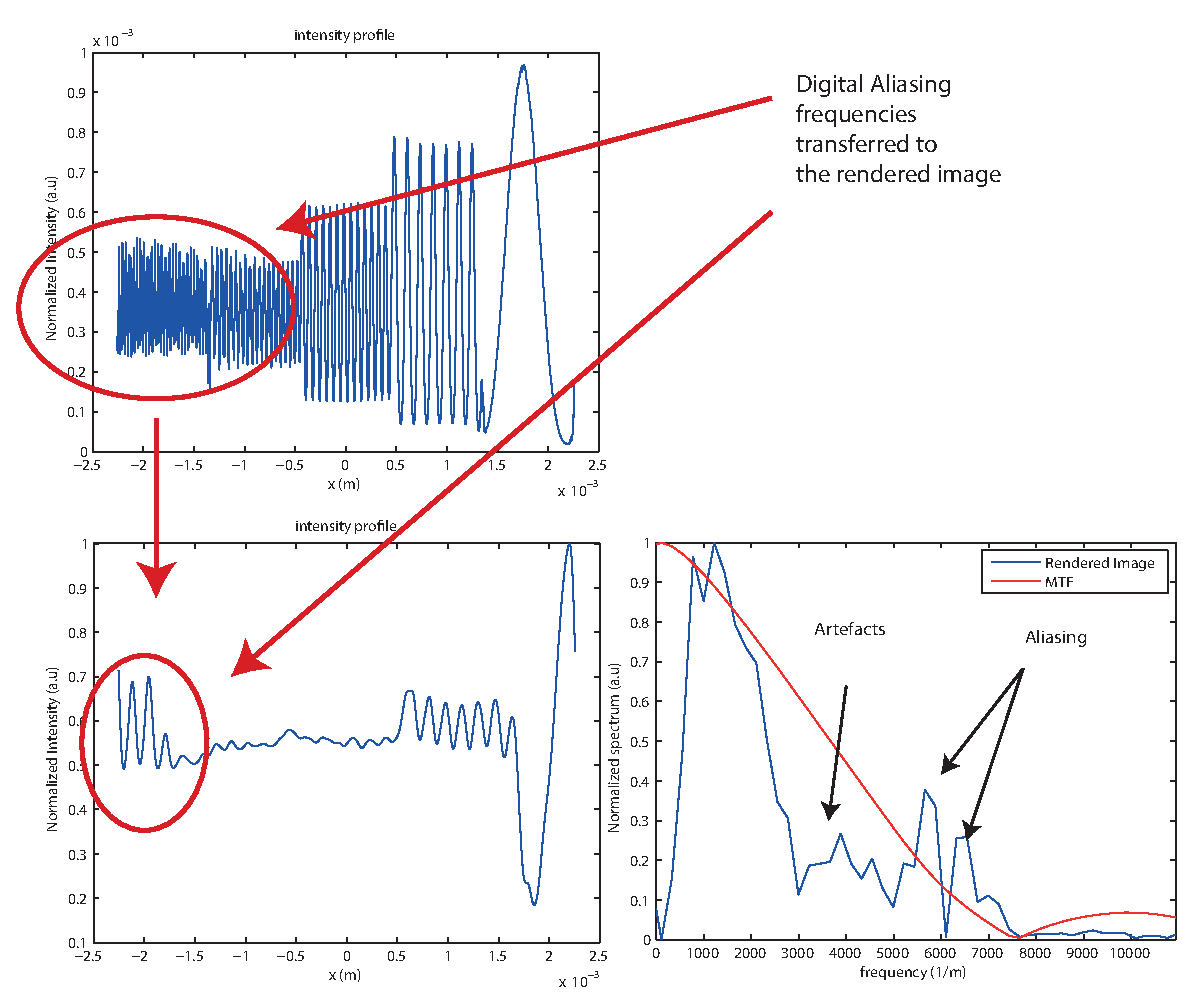
\includegraphics[width=1\textwidth]{C:/Users/Massimo/Documents/Thesis/aliasing.eps}.
 	\caption{\label{fig:aliasing} Aliased frequencies transmitted to the rendered image. }
 \end{figure}
If the magnification is \textit{0.25} the situation becomes the one in figure \ref{fig:image025} and figure \ref{fig:freq025}.
 \begin{figure}[H]
 	\centering
 	\includegraphics[width=1\textwidth]{C:/Users/Massimo/Documents/Thesis/images025.eps}.
 	\caption{\label{fig:image025} Top: raw sensor image, on the right the main lens image. Bottom: On the left there is the  rendered image, on the right the same image has been low pass filtered to remove some of the rendering artefacts. Magnification was 0.3.  }
 \end{figure}
 \begin{figure}[H]
 	\centering
 	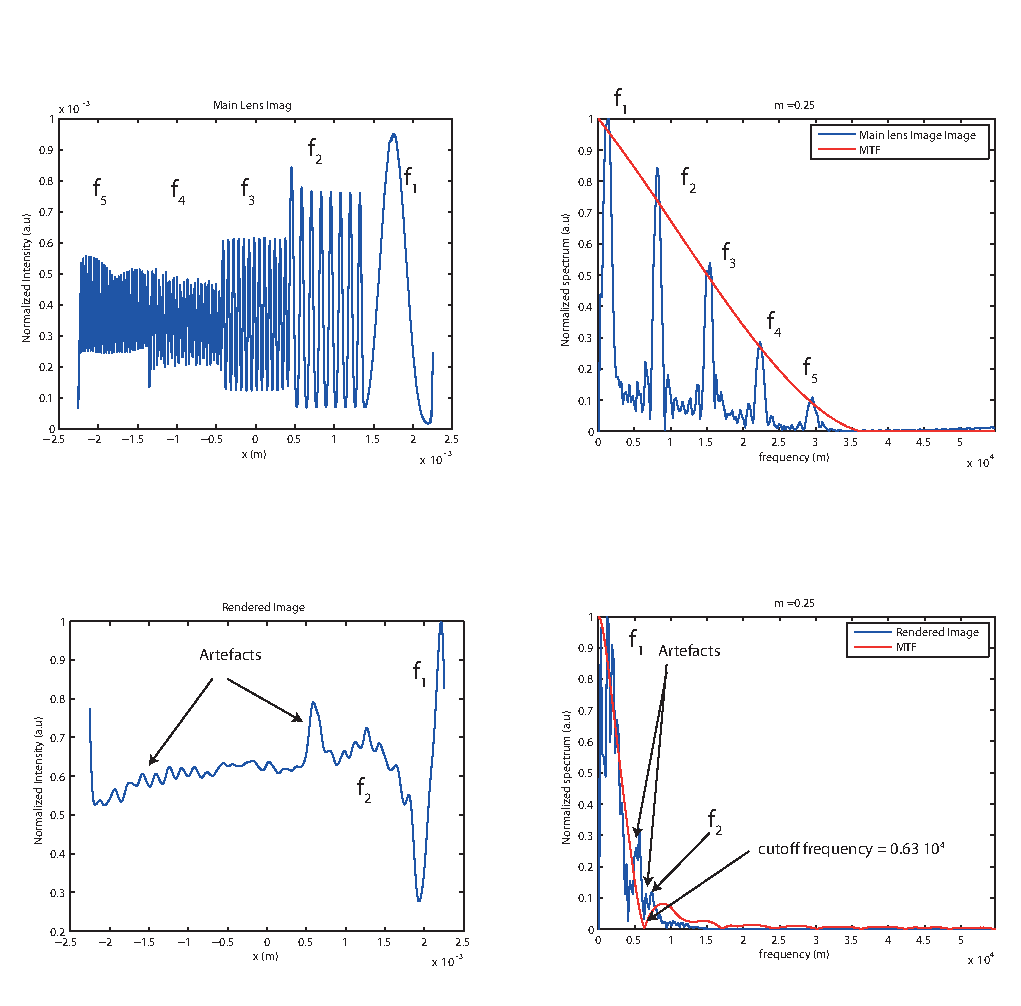
\includegraphics[width=1\textwidth]{C:/Users/Massimo/Documents/Thesis/MTF025final2.eps}.
 	\caption{\label{fig:freq025} On the left: intensity profiles of the main lens image, top and of the rendered image,bottom.On the right there are the spatial frequencies modulated according to the MTF. The first zero frequency of the system is $0.6 \times 10^4 1/m$} 
 \end{figure}
 In the results shown in figure \ref{fig:freq025} there is a lower magnification and the digital aliasing frequencies are no longer transmitted to the rendered image. This is due to the fact that with a narrower  bandwidth of the modulation transfer function these frequencies are filtered out of the signal. The same happens to the frequency $f_2$ of the object field, since the cut off frequency for a magnification equal to 0.25 is lower that the signal frequency $f_2$.
 \section{Conclusions}
 In this chapter a frequency analysis of a focused plenoptic system has been done to investigate its behaviour at its diffraction limit. The optical performances of the plenoptic imaging system were analysed. It was treated as a linear system with a finite bandwidth that depends on the magnification of the lenslet array. The distances \textit{a} and \textit{b} not only define the angular resolution of the system and the trade off with spatial resolution, but also allows to quantify the limits of the system in terms of optical resolution. This is a new contribution to the field, first presented in 2014 \cite{turola2014wave}.  Knowing how the optical frequencies are transmitted though the system allows to design its components in order to satisfy the requirements imposed by the practical application encountered. The optical resolution degradation with increase of the angular resolution represents an intrinsic limitation to plenoptic 2.0 imaging system especially in applications regarding microscopy in which it is the diffraction that limits the resolution.\\
 There are three ways to overcome this limitations: optically, computationally and a hybrid one. The first approach consists in improving the basic optical elements of the system, that is choosing low f-number optical elements, larger arrays of micro lenses and sensors, or improving the optics before the micro array stage in order to deliver pre processed optical frequencies that will not be affected by the loss of resolution in the relay stage. It is also possible to act on the micro lens array, creating an array of lenslets with different focal lengths \cite{georgiev2012multifocus}. This approach could result in expensive devices, and it is preferable to approach this issue computationally.  Raw plenoptic data can be treated in post processing and can lead to a full sensor resolution rendering, and even a super resolution rendering as done by Georgiev \textit{ et al.} \cite{georgiev2009superresolution,georgiev2012super,georgiev2011superresolution,georgiev2015plenoptic,georgiev2009high}, by Favaro and Bishop \cite{favaro2012split,bishop2012light,bishop2011full,bishop2009light} and Shroff \textit{et al.} \cite{shroff2012high,shroff2013image}. Another way to overcome the loss of resolution is to design a hybrid system composed of two branches, a plenoptic branch and a conventional high resolution branch. These hybrid systems \cite{lu2013high,boominathan2014improving}, are based on the simultaneous acquisition of a plenoptic and a high resolution image, the latter being used as a base to interpolate the plenoptic data in order to fill the gaps in resolution.\\
 In the next chapter the knowledge and the experience acquired designing and testing simulated plenoptic imaging systems through simulation will be used to design and build a laboratory optical setup, and the results obtained will be discussed.
 \nomenclature{$\delta x$}{Rayleigh distance}
 \nomenclature{$h$}{Impulse response}
 \nomenclature{$H$}{Optical transfer function}

   

 